\documentclass[14pt]{extarticle}
\usepackage[utf8]{inputenc}
\usepackage[T1]{fontenc}
\usepackage[spanish,es-lcroman]{babel}
\usepackage{amsmath}
\usepackage{amsthm}
\usepackage{physics}
\usepackage{tikz}
\usepackage{float}
\usepackage[autostyle,spanish=mexican]{csquotes}
\usepackage[per-mode=symbol]{siunitx}
\usepackage{gensymb}
\usepackage{multicol}
\usepackage{enumitem}
\usepackage[left=2.00cm, right=2.00cm, top=2.00cm, 
     bottom=2.00cm]{geometry}

%\renewcommand{\questionlabel}{\thequestion)}
\decimalpoint
\sisetup{bracket-numbers = false}

\title{\vspace*{-2cm} Ejercicios de Velocidad \\  Evaluación Continua - Física III\vspace{-5ex}}
\date{}

\begin{document}
\maketitle

\textbf{Indicaciones:} Resuelve de manera detallada cada uno de los siguientes ejercicios, en donde deberás de indicar el paso (o pasos necesarios) para llegar al resultado, en el caso de las conversiones de unidades, deberás de anotar el(los) factor(es) de conversión necesarios.
\par
Al inicio de cada hoja que utilices para tu solución, deberás de anotar tu nombre completo.
\par
Esta actividad otorga hasta \textbf{10 puntos}. Si se reporta el resultado directo, sin presentar el desarrollo del ejercicio, éste no aporta puntaje.
\par
La solución se deberá de enviar por Teams (ya sea en foto o la hoja escaneada).

\section*{Ejercicios a resolver.}

\begin{enumerate}
\item ¿A qué distancia (en metros) viaja hacia adelante un automóvil que se mueve a razón de 55 millas/h durante \SI{1}{\second} de tiempo, que es lo que le toma ver un accidente al lado de la carretera?
\item El lanzador de los Medias Rojas de Boston, Roger Clemens, lanzó una bola rápida a una velocidad horizontal de \SI{160}{\kilo\meter\per\hour}, según fue verificado con una pistola de radar. ¿Qué tanto le tomó a la bola llegar a la base de meta, que está a una distancia de \SI{18.4}{\meter}?
\item ¿A qué velocidad promedio iba un auto que recorrió \SI{250}{\kilo\meter} en \SI{3}{\hour}?
\item ¿A qué velocidad en \unit{\kilo\meter\per\hour} corrió Usain Bolt en el Campeonato Mundial de Berlín en el año 2009 para batir el récord mundial de los \SI{100}{\meter} planos en \SI{9.58}{\second}?
\item ¿Qué distancia recorrió un avión que viajaba a \SI{750}{\kilo\meter\per\hour} después de \SI{2.5}{\hour} de vuelo?
\item Calcula la velocidad en \unit{\kilo\meter\per\hour}, a la que corrió el atleta keniata Wilson Kipsang Kiprotich para batir el récord mundial vigente, que realizó en el maratón de Berlín, en el año 2013, cuya distancia total es de \SI{42.195}{\kilo\meter}, en un tiempo de \SI{2}{\hour} \SI{3}{\minute} \SI{23}{\second}.
\item En la siguiente gráfica se muestra el desplazamiento en función del tiempo para cierto objeto que se mueve a lo largo del eje $x$.
\begin{figure}[H]
    \centering
    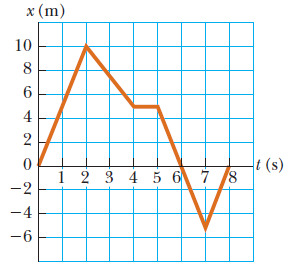
\includegraphics[scale=1]{Imagenes/Ejercicio_Cuenta_01.png}
\end{figure}
Encuentra la velocidad en los siguientes intervalos de tiempo:
\begin{enumerate}[label=\alph*)]
\item \num{0} a \SI{2}{\second}
\item \num{0} a \SI{4}{\second}
\item \num{2} a \SI{4}{\second}
\item \num{4} a \SI{7}{\second}
\item \num{0} a \SI{8}{\second}
\end{enumerate}
\item Un motociclista adquiere una velocidad de \SI{50}{\kilo\meter\per\hour} en \SI{6}{\second}. ¿Cuál es su aceleración en \unit{\meter\per\square\second}?
\item Un camión lleva una velocidad inicial de \SI{6}{\meter\per\second}, a los \SI{4}{\second} su velocidad es de \SI{8}{\meter\per\second}. Calcula su aceleración.
\item  Un avión vuela en la misma dirección y sentido a \SI{860}{\kilo\meter\per\hour} durante un tiempo de \SI{20}{\minute}. ¿Cuál es su aceleración durante ese intervalo de tiempo y por qué?
\end{enumerate}
\end{document}